


  \section{Theorie}
Ziel des Versuchs ist die Bestimmung des Verhältnisses zwischen h und $\symup{e_0}$.
Der Photoeffekt ist ein Beweis für den Teilchencharakter von Licht.
\subsection{allgemeiner Photoeffekt}
Ein prinzipieller Versuchsaufbau ist in Abbildung \ref{fig:prinz} zu sehen.\\
\begin{figure}
  \centering
  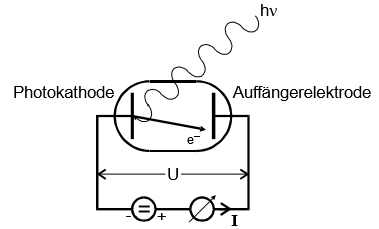
\includegraphics[scale=0.7]{prinzipschaltung.png}
  \caption{Prinzipielle Anordnung zur Untersuchung des Photoeffektes}\cite{Anleitung}
  \label{fig:prinz}
\end{figure}

Die Photokathode wird mit Licht bestrahlt und Elektronen treten aus.
Dabei kann ein Photon höchstens ein Elektron auslösen.\\
Aus der prinzipiellen Untersuchung des Photoeffekts ergibt sich,
dass die Zahl der ausgelösten Elektronen proportional zur Lichtintesität ist
und dass die Energie der Photoelektronen proportional zur Lichtfrequenz und
unabhängig von der Lichtintensität ist.
Außerdem existiert eine Grenzfrequenz.
Unterhalb dieser Frequenz kann der Photoeffekt nicht ausgelöst werden.
Diese Ergebnisse lassen sich nicht mit dem Wellenbild erklären.
Darum wird nun vom Teilchenmodell ausgegangen und
dass die Energie von Photonen, den Lichtquanten, transportiert wird.
Aus dieser Annahme folgt nun, dass ein Photon die Energie $\symup{h\nu}$ besitzt.
Die Energie eines Photons,
die beim Verlassen des Metalls
 momentan auf ein Elektron übertragen wird
teilt sich in die Austrittsarbeit $\symup{A_k}$ und die kinetische Energie auf.

\begin{equation}
  h\nu = E_{\symup{kin}} + A_k
\end{equation}
Damit der Photoeffekt auftritt, muss die Energie größer als die Austrittsarbeit sein.
\subsection{experimentelle Untersuchung des Photoeffktes mit Photozelle}

In Abbildung (\ref{fig:pk}) ist eine Photokathode zu sehen,
die im durchzuführenden Versuch verwendet wird.
In ihr findet die Auslösung der Eletronen statt.
\begin{figure}[H]
  \centering
  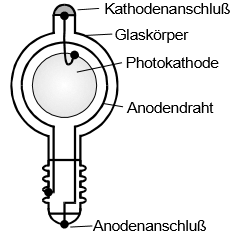
\includegraphics[scale=0.7]{bild2.png}
  \caption{Die Photozelle}\cite{Anleitung}
  \label{fig:pk}
\end{figure}

\begin{figure}
  \centering
  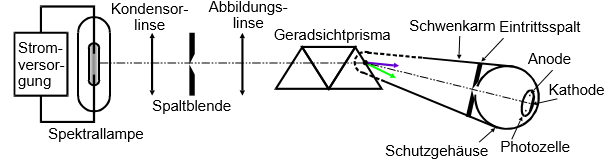
\includegraphics[scale=0.7]{bild3.png}
  \caption{Versuchsaufbau}\cite{Anleitung}
  \label{fig:ver}
\end{figure}

Der hier verwendete Versuchsaufbau ist in Abbildung (\ref{fig:ver}) zu sehen.
Mit Hilfe dieser Apparatur wird das Licht in seine einzelnen Spektrallinien aufgeteilt.
Die einzelnen Farben besitzen unterschiedliche Wellenlängen.
Durch den Schwenkarm ist es möglich die unterschiedlichen Farben,
also das monochromatische Licht, einzeln zu messen.
An die Strecke zwischen Kathode und Anode wird eine Spannung U angelegt.
Dadurch wird ein elektronen-abbremsendes Feld erzeugt.
Der zu messende Strom verschwindet, wenn gilt:
\begin{equation}
  e_0 U_g = \frac{1}{2} m_0 V^2_{\symup{max}}
\end{equation}
Dabei ist $\symup{e_0}$ die Elementarladung, $\symup{m_0}$ die Ruhemasse,
$\symup{v_{max}}$ die Geschwindigkeit der schnellsten Elektronen und $\symup{U_g}$ eine Gegenspannung und Grenzspannung.
Daraus folgt also der Zusammenhang
\begin{equation}
  h\nu = e_0 U_g + A_k
\end{equation}
Ist die Bremsspannung U gleich der Grenzspannung $\symup{U_g}$ veschwindet der Photostrom nicht schlagartig.
Er sinkt schon für Werte, die größer sind als $\symup{U_g}$.
Das liegt daran, dass die Photoelektronen nicht monoenergetisch sind.
Sie bestitzen eine Energieverteilung von 0 bis $\symup{(\sfrac{1}{2})mv^2_{max}}$.\\
Über diese Energieverteilung macht die Fermi-Dirac-Statistik eine Aussage.
Laut dieser ist es möglich, dass Elektronen austreten, deren Energie größer ist als
$\symup{h\nu - A_k}$.\\
Nicht alle Photoelektronen erreichen die Anode nach verlassen der Kathode.
Das liegt zum einen daran, dass die Oberfläche viel zu klein ist.
Zum anderen an der hohen Austrittsarbeit $\symup{A_A}$ des Anodenmetalls.
Es tritt kein Photostrom auf wenn $\symup{h\nu < A_A}$

In Abbildung \ref{fig:iu} ist der Photostrom in Abhängigkeit von der Bremspannung aufgetragen.
\begin{figure}
  \centering
  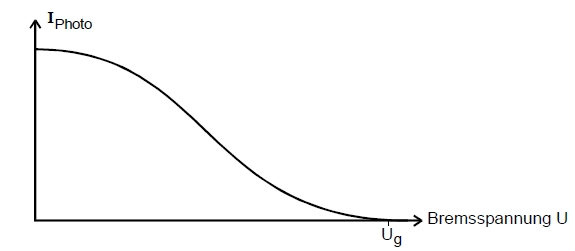
\includegraphics[scale=0.7]{kurv.jpg}
  \caption{Photostrom in Abhängigeit von der Bremsspannung in einer mit monochromatischem Licht bestrahlte
  Photozelle}\cite{Anleitung}
  \label{fig:iu}
\end{figure}
Um den Punkt $\symup{U_g}$ wird die Funktion quadratisch genährt,
sodass unter bestimmten Vorraussetzungen ein parabolischer Zusammenhang zwischen dem Photostrom
und der Bremsspannung besteht.

  \section{Durchführung}
Zunächst werden die Aufbauten so eingestellt,
dass die einzelnen Farben den Schlitz, der zur Photozelle führt, komplett überdecken.

  Im ersten Teil des Versuchs wird für unterschiedliche Spannungen
  und Farben der Photostrom gemessen.
  Die Spannung wird im Bereich von -2V bis +2V gewählt.
  Es werden die Farben orange, grün, blau, grün-blau
  und zwei lila Farben für zwei unterschiedliche Wellenlängen gemessen.\\
  Die Messung wird für zehn unterschiedliche Spannungen durchgeführt.
Die ungefähren Wellenlängen sind in tabelle \ref{tab:wel} zu finden.
\begin{table}
\centering
\caption{Berechnete Frequenzen}
\label{tab:wel}
\begin{tabular}{c c }
\toprule
{Farbe} & {Wellenlänge in nm} \\
\midrule
orange & 587,6 \\
grün & 501,6 - 504,8 \\
grün-blau & 492,2 \\
blau & 471,3 \\
lila & 447,1 \\
lila & 438,8\\
\bottomrule
\end{tabular}
\end{table}

  Im zweiten Teil des Versuchs wird das gelbe Licht eingestellt,
  bei ca. 578nm.
  Es wird wieder der Photostrom gemessen.
  Diesmal wird die Beschleunigungsspannung zwischen -5 bis +20V eingestellt.
